\chapter{Data and computational methodology}
\section{Data provenance}
The input is a 10-column text table with \num{300003} numerical rows. Its SHA256 and the hash of the original script are recorded in the inventory. The original materials are retained unchanged. The table contains scalar descriptors and a column labelled \code{metad.rbias}. Contact maps or molecular renderings would additionally require atomic coordinates and a verified mapping from each row to its structural frame.

The paper and the script serve different purposes in the audit. The publisher PDF describes the method to reproduce; the supplied source shows how that method was implemented. Execution evidence is needed to determine whether an analysis actually completed. Scientific V2 and its changelog were unavailable, so their contents remain an explicit gap in the method map.

\section{Replica segmentation}
Replica boundaries are detected where the first column decreases. Parsing requires exactly three segments, strictly increasing times within each segment, finite numerical entries, and a recognized header. Extra segments, duplicate times, malformed rows, or missing interval coverage fail validation rather than being silently skipped.

Frame identities are preserved before any selection or shuffling: zero-based source row, one-based file line, replica ID and zero-based frame index within its original segment. A partition comparison then matches the same observations across runs. Comparing arrays in their current storage order would otherwise confuse a reordering of frames with a change in the clustering.

\section{Analysis interval}
The baseline interval includes both endpoints from \num{1000000} to \num{3000000} in the source-labelled picosecond time unit. Each replica contributes \num{100001} frames separated by 20 ps. The original script and published protocol support this unit interpretation, but the upstream simulation/analysis metadata are absent. The interval therefore corresponds to the supplied 1--3 μs window under a recorded provenance assumption.

The published workflow excludes the first microsecond. The supplied table already begins at the selected boundary, so it permits verification of interval coverage but cannot support an independent assessment of the preceding equilibration period or the full-trajectory convergence analysis.

\section{Descriptor definitions}
The canonical clustering columns are $\na$, $\nb$, $R_g$ in nm, and SASA in nm$^2$, with units inherited from the original script. Header spelling differences are mapped explicitly, including the original \code{HBONNDSPS} spelling. The \code{metad.rbias} column is preserved as a separate field and is not renamed to an interpolated free energy.

The FES and the clustering algorithm use different coordinates. FES queries apply the paper's descriptor conversions, $\alpha=\na/1.1$ and $\beta=\nb/2.5$, whereas clustering uses normalized features. Passing min--max-scaled values to the FES would select different physical CV locations. Separate modules and saved parameters keep these transformations distinct.

\section{Feature normalization}
For each baseline descriptor $x_f$, pooled analysis-window min--max scaling gives $z_f=(x_f-a_f)/(b_f-a_f)$, where $a_f$ and $b_f$ are the pooled minimum and maximum. Both values are saved. A constant feature is an invalid input for this transform, rather than a reason to divide by zero or silently remove a scientific variable.

The pooled transform gives every replica and discovery group the same coordinate system. If each group were scaled independently, an observation's numerical position would depend on the group to which it had been randomly assigned. The baseline therefore retains the source's common min--max scaling. Standardization belongs to the separate GMM protocol; the planned DPC scaling comparisons remain unperformed.

\section{STEP 1: iterative Density Peak Clustering}
The workflow in \cref{fig:workflow} begins with random disjoint subsets. Production group size is approximately \num{30000}. A tiny final subset of at most ten frames is redistributed over preceding groups, preserving every identity. Local RNG streams are derived from a recorded master seed. This removes the legacy fixed-seed-list limit, but changes exact random draws relative to the original global-RNG implementation \autocite{numpyrng}.

Local density is the number of neighbors within $d_c$, including the point itself as in the supplied code. To handle equal densities reproducibly, points are ordered by density and then by local frame position. The separation $\delta_i$ is measured to the closest earlier point in that order; the first point uses the maximum pairwise distance. Ranking $\rho_i\delta_i$ then identifies candidate centers that combine density with separation. The tie rule matters because an earlier point need not be strictly denser.

For each cutoff, candidate center counts are scanned from 10 down to 2. The selected candidate maximizes the number of acceptable clusters; ties retain the earlier, higher-center-count candidate. Acceptance requires at least 300 members and mean silhouette at least 0.3. After accepted members are removed, $d_c$ is multiplied by 0.9. The process stops when fewer than 300 points remain or five consecutive iterations accept no cluster. Residual points remain unassigned at this stage.

\begin{figure}[tb]
\centering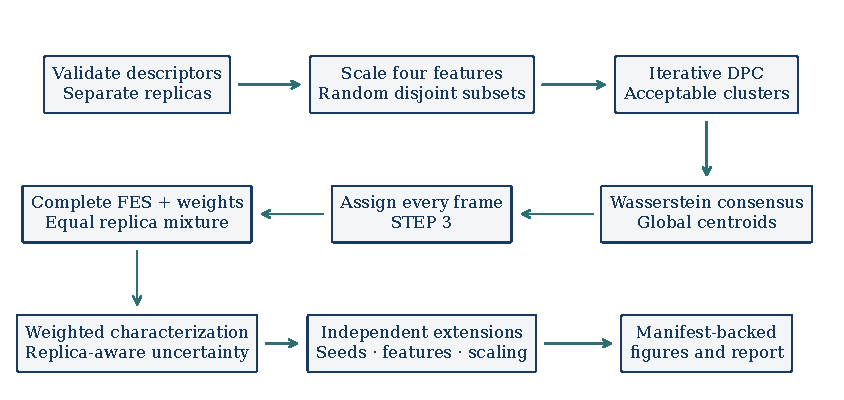
\includegraphics[width=\textwidth]{fig01_workflow.pdf}
\caption{Implemented analysis design. The primary branch separates geometric cluster discovery from statistical reweighting. Robustness experiments rerun designated stages independently. The FES grid has been validated, while empirical weighting remains blocked by energy-unit and construction provenance; this workflow diagram documents implementation, not successful completion of every box.}
\label{fig:workflow}
\end{figure}

Distances are computed in bounded blocks into a float32 matrix. Cutoff density is evaluated row by row without an additional floating kernel matrix. Silhouettes reuse that distance matrix, subject to the validity condition that the number of labels lies between two and $N-1$ \autocite{sklearnsilhouette}. The algorithm still has quadratic storage and potentially substantial repeated silhouette cost; the changes reduce avoidable allocations rather than changing its asymptotic scaling.

\section{STEP 2: Wasserstein consensus}
Only acceptable local clusters enter consensus. For clusters $A$ and $B$, the implemented source metric is
\begin{equation}
D(A,B)=\left[\sum_{f=1}^{4}W_1(A_f,B_f)^2\right]^{1/2}.
\label{eq:wasserstein}
\end{equation}
Here $W_1$ is the one-dimensional first Wasserstein distance between empirical marginal descriptor distributions \autocite{scipywasserstein}. Equation~\ref{eq:wasserstein} does not describe joint four-dimensional optimal transport. It can miss changes in dependence structure that leave every marginal distribution unchanged.

The reproduction configuration uses raw descriptors, matching the supplied code. This mixes descriptor scales and units in the aggregate norm; the paper does not fully resolve that scaling choice. The normalized alternative is retained as an explicit extension. Average-linkage agglomeration is followed by the source's cubic-spline elbow heuristic: smoothing parameter 5, with the maximum second derivative sought in the first 90\% of merge steps. Fewer than five local clusters or an entirely flat merge-height curve yields an explicit failure instead of an invented cut.

\section{STEP 3: final frame assignment}
Each global centroid is the mean normalized feature vector of all accepted local-cluster members assigned to that family. All analysis-window frames, including residuals and frames outside reduced discovery groups, are assigned once to the nearest centroid. Distance ties use deterministic label ordering. Centroids are not iteratively refitted after reassignment: doing so would introduce a k-means refinement absent from the documented baseline.

The final labels are stored with the original frame identities. This lets descriptor statistics, stability comparisons and any later structural mapping refer to exactly the same observations. Their molecular interpretation remains limited by the chosen descriptor representation.

\section{FES validation and interpolation}
The FES parser requires explicit axis names, extrema, grid counts, and nonperiodic status. It verifies row count, finite values including supplied derivative columns, coordinate spacing, unique Cartesian pairs, and agreement with the header. Row order is not assumed. A partial-download extension is rejected before parsing.

Interpolation uses SciPy's linear rectilinear-grid interpolator with bounds checking enabled \autocite{scipygrid,virtanen2020}. Every query must fall inside both axes. A bilinear analytic surface containing a mixed $\alpha\beta$ term provides an exact test, including boundary queries and shuffled rows. Missing cells and out-of-bounds queries are errors; no extrapolation or clipping is permitted.

\section{Statistical weights}
Equation~\ref{eq:finalweights} is evaluated in log space. Within replica $r$, normalized weights are
\begin{equation}
\widetilde w_{ri}=\exp\!\left[\ell_{ri}-\operatorname{logsumexp}_j(\ell_{rj})\right],
\qquad W_{ri}=\frac{\widetilde w_{ri}}{3}.
\label{eq:replicaweights}
\end{equation}
Equation~\ref{eq:replicaweights} gives each replica equal total mass, independently of the arbitrary log-weight offset or differences in raw weight sums. The recorded raw exponential is diagnostic only. If it is not representable, the output includes an explicit overflow/underflow status; normalized calculations remain based on log weights.

The intended frame table contains replica, source row, file line, frame index, time, physical CVs, interpolated free energy, raw log weight, raw weight/status, within-replica weight, pooled weight, and final label. No such real weighted table is reported in this release because FES energy-unit and construction provenance remain unverified.

\section{Weighted cluster characterization}
For a cluster, summing the pooled weights gives its relevance. Restricting those weights to its members gives the conditional descriptor mean and width. The width is the square root of the weighted central second moment: it describes heterogeneity within the family. Replica SEM addresses a different question, the variation of the relevance estimate across replicas, and is calculated from the separate replica populations.

The uncertainty extension keeps the fitted labels and supplied FES fixed while resampling contiguous observation blocks independently within each replica. It renormalizes the selected weights and recalculates populations for each draw. The resulting intervals would be conditional on that partition and FES; they do not incorporate uncertainty from reconstructing the FES, selecting a model or changing the clustering seed. This scope is recorded with the output.

\section{Software environment and reproducibility}
The modular implementation uses NumPy, SciPy, pandas, Matplotlib and scikit-learn; the key numerical and machine-learning libraries have established primary descriptions \autocite{harris2020,virtanen2020,pedregosa2011}. A locked environment records installed versions separately from published simulation versions. Snakemake expresses stage dependencies, while CLI commands provide the same functionality without notebooks \autocite{snakemakedocs,wratten2021}.

Each run begins with a manifest and resolved parameters. A supervisor records the worker's status and samples process-tree memory every 0.1 s, enforcing configured runtime and memory limits. Successful, failed, and blocked runs have distinct final statuses. Figures may be rebuilt only from a successful manifest after its output hashes are checked. The resulting record links each figure to the calculation and data that produced it.
